\RequirePackage{luatex85}
\documentclass{article}
\usepackage{tikz, amsmath, mathtools, multicol, setspace}
\setlength\parindent{0mm}
\thispagestyle{empty}
\pagestyle{empty}
\everymath{\displaystyle}

% define macro \Repeat{integer}{content}
\usepackage{expl3}
\ExplSyntaxOn
\cs_new_eq:NN \Repeat \prg_replicate:nn
\ExplSyntaxOff

\newcommand\blob[2][15mm]{\(\begin{matrix}\begin{tikzpicture}
	\node[text width=#1, align=flush center]{\begin{spacing}{0.7}#2\end{spacing}};
	\end{tikzpicture}\end{matrix}\)}
\newcommand\myoverset[2]{\smash{\large$\overset
	{#1}{\vphantom{\bigg(}\hspace{#2mm}}
	$}}

\usepackage[margin=0.5in, column sep=1in]{geometry}

\begin{document}
\large

\Repeat{2}{
% margin=0.5in, row sep=1in, so textheight=4.5in
\begin{minipage}[t][4.5in]{\textwidth}
\section*{The Limit Definition of Derivative}

\vspace{-1ex}
Suppose the height of a ball is a function of time $y=f(x)$.

\bigskip\hfil
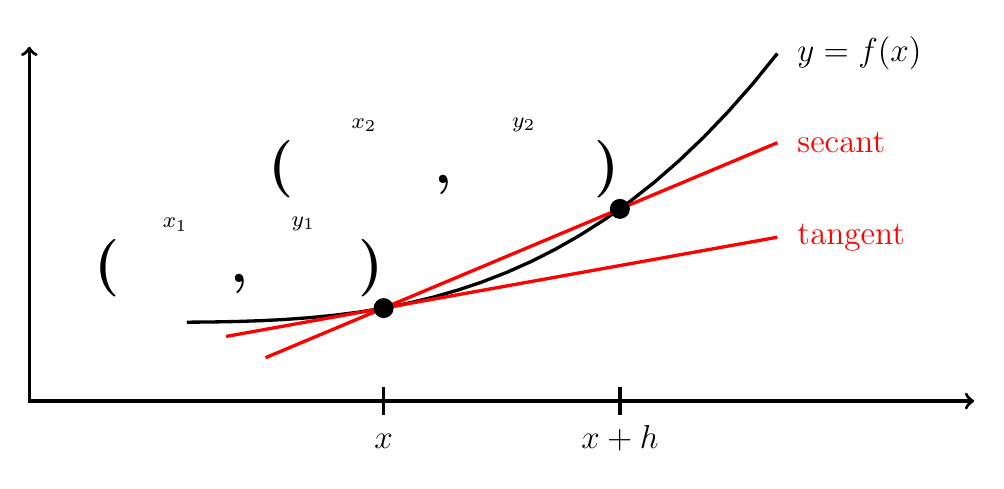
\begin{tikzpicture}[very thick]
	% axes
	\draw[<->] (-1.5,4.5) to (-1.5,0) to (10.5,0);
	% f(x)
	\draw[domain=0.5:8] 
		plot (\x, \x^3/150+1) node [right] {\,\,\large$y=f(x)$};
	% secant
	\draw[red, domain=1.5:8] 
		plot (\x, {3^3/150+1+(\x-3)*(6^3-3^3)/(6-3)/150})
		node [right] {\,\,\large secant};
	% tangent
	\draw[red, domain=1:8] plot (\x, {3^3/150+1+(\x-3)*3^2*3/150})
		node [right] {\,\,\large tangent};
	% closed circles
	\foreach \x/\n in {3/x,6/x+h}{
		\draw[black, fill=black] (\x, \x^3/150+1) circle (3pt) coordinate (\x);
		\draw (\x, 5pt) -- ++(down:10pt) node[below] {\large$\n\vphantom h$};
		}
	% fillin (x1, y1) = (x, f(x))
	\draw (3) node [above left] {
		\bfseries\huge(\myoverset{x_1}{14},\myoverset{y_1}{14})\!
		};
	% fillin (x2, y2) = (x+h, f(x+h))
	\draw (6) node [above left] {
		\bfseries\huge(\myoverset{x_2}{18},\myoverset{y_2}{18})\!
		};
	\end{tikzpicture}

\vfill
\blob{avera\smash ge velocity over $[x, x{+}h]$}
= \blob{avera\smash ge rate of change over $[x, x{+}h]$}
= \blob{slope of secant between $x, x{+}h$}
=\hfill$\frac{\Delta y}{\Delta x}$\hfill%
=\hfill$\frac{y_2 - y_1}{x_2 - x_1}$\hfill%
=\hfill{\LARGE\boxed{\phantom{\frac{f(x+h)-f(x)}h}}}\hfill%
= \blob[22mm]{definition of difference quotient}

\vfill
\blob{velocity at $x$}
= \blob{rate of change at $x$}
= \blob{slope of tangent at $x$}
=\hfill{\LARGE\boxed{\lim_{h\to\quad}\phantom{\frac{f(x+h)-f(x)}h}}}\hfill%
=\hfill\!definition of derivative $f'(x)$

\vfill
\end{minipage}

\vspace{1in}
}
\end{document}
